\chapter{Descriptive Statistics}

\section{CPU Data}
\begin{figure}[p]
  \centering
  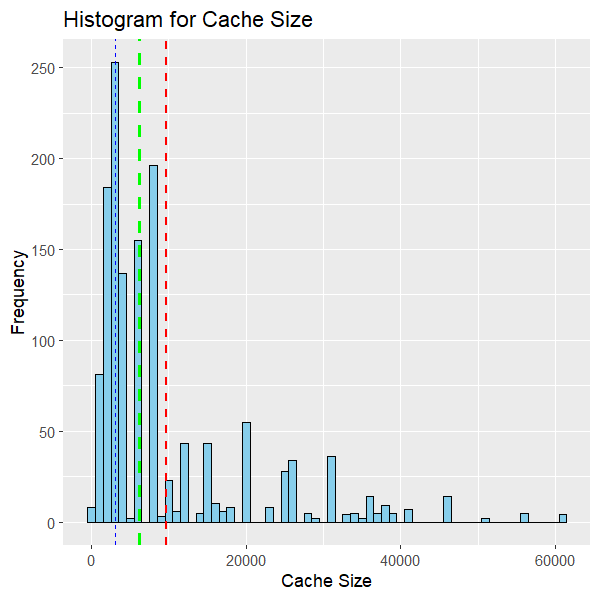
\includegraphics[width=0.33\linewidth]{img/CPU_histo_Cache.png}\hfill
  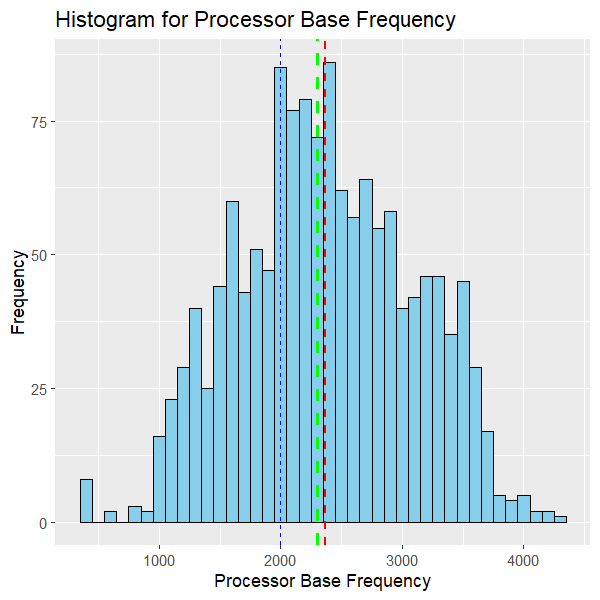
\includegraphics[width=0.33\linewidth]{img/CPU_histo_Freq.png}\hfill
  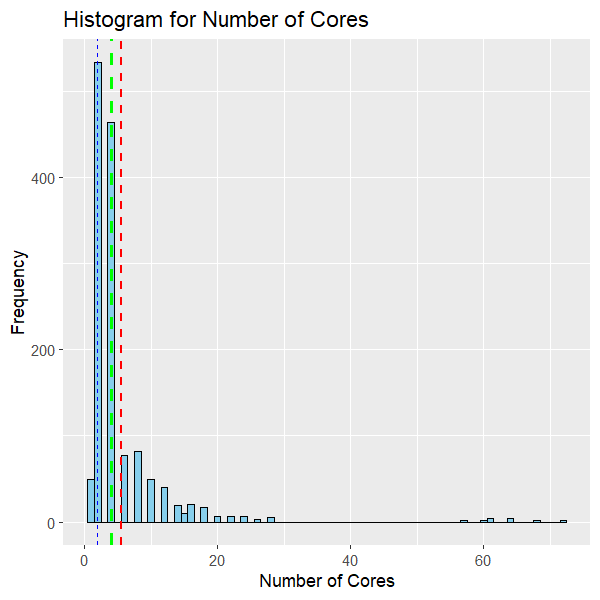
\includegraphics[width=0.33\linewidth]{img/CPU_histo_Core.png}
  \\[\smallskipamount]
  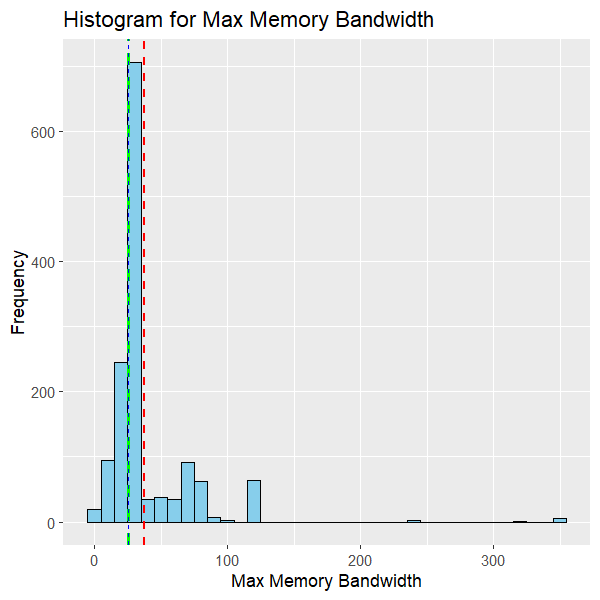
\includegraphics[width=0.33\linewidth]{img/CPU_histo_MMB.png}\hfill
  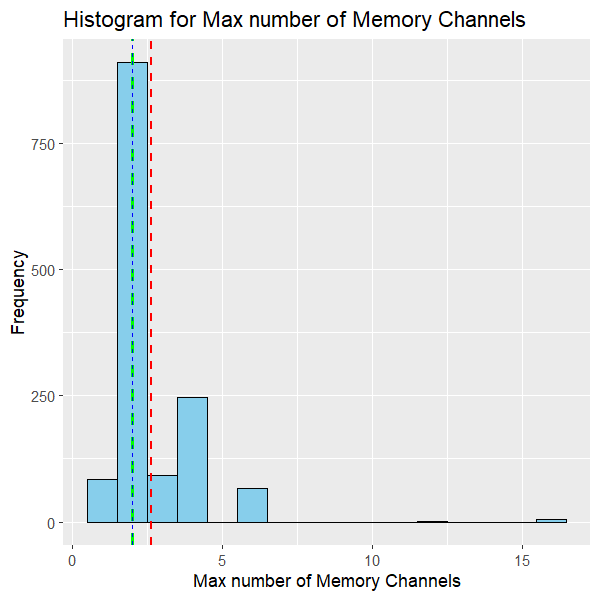
\includegraphics[width=0.33\linewidth]{img/CPU_histo_MNMC.png}\hfill
  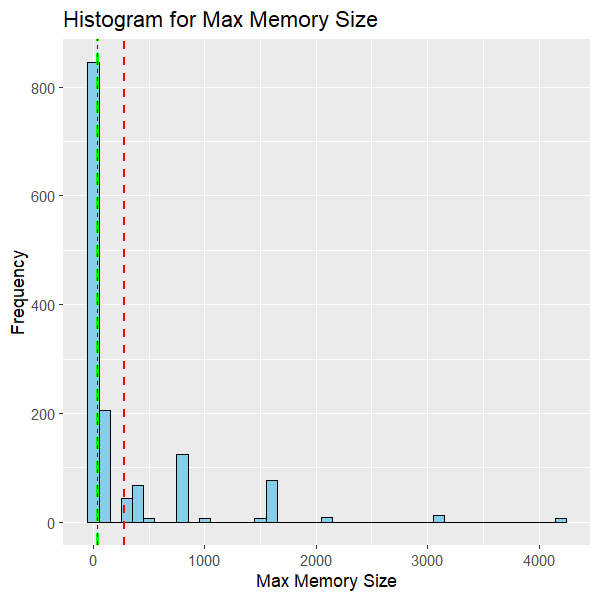
\includegraphics[width=0.33\linewidth]{img/CPU_histo_MMS.png}
  \\[\smallskipamount]
  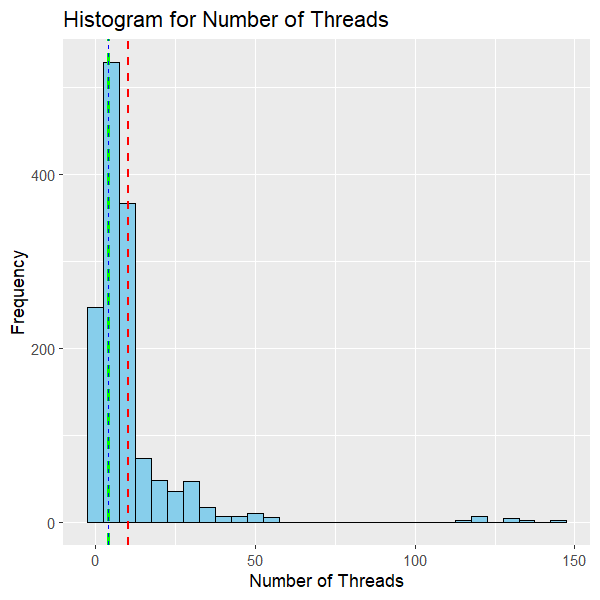
\includegraphics[width=0.33\linewidth]{img/CPU_histo_Thread.png}\hfill
  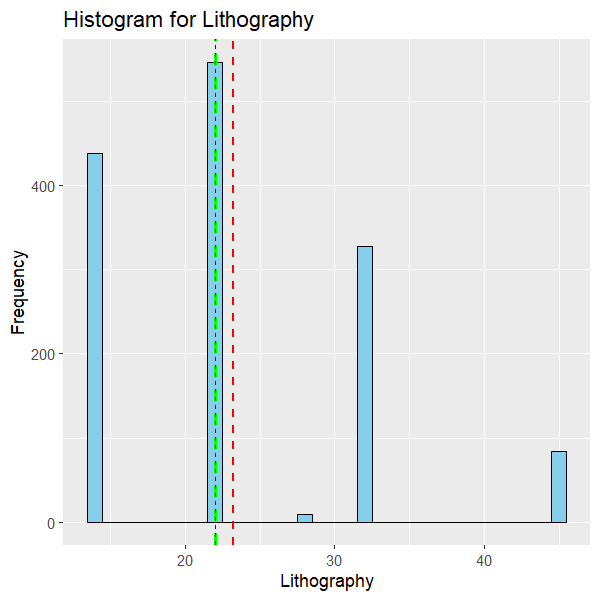
\includegraphics[width=0.33\linewidth]{img/CPU_histo_Litho.png}\hfill
  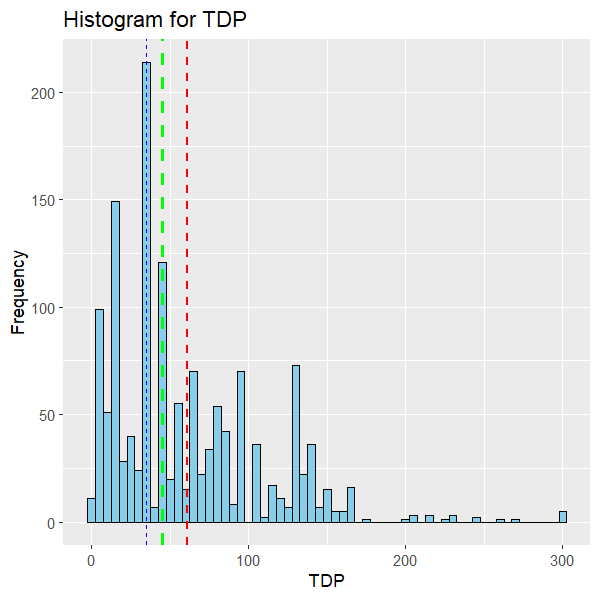
\includegraphics[width=0.33\linewidth]{img/CPU_histo_TDP.png}
  \vspace{10pt}
  \caption{Histograms of several features in CPU data}
  \label{fig:Na_GPU}
\end{figure}


\begin{lstlisting}[language=R]
litho_year <- CPUs_processed %>% 
  group_by(Release_Year) %>%
  summarize(mean_litho = mean(Lithography),
            median_litho = median(Lithography),
    .groups = "drop"
  )

ggplot(litho_year, aes(x = Release_Year)) +
  geom_line(aes(y = mean_litho, color = "Mean")) +
  geom_line(aes(y = median_litho, color = "Median")) +
  scale_color_manual(values = c("Mean" = "blue", "Median" = "red")) +
  labs(x = "Year", y = "Lithography", title = "Mean and Median Lithography by Year") +
  scale_x_continuous(breaks = seq(min(litho_year$Release_Year), max(litho_year$Release_Year),
  by = 1)) +
  theme_minimal()
\end{lstlisting}

\begin{figure}[ht]
  \centering
  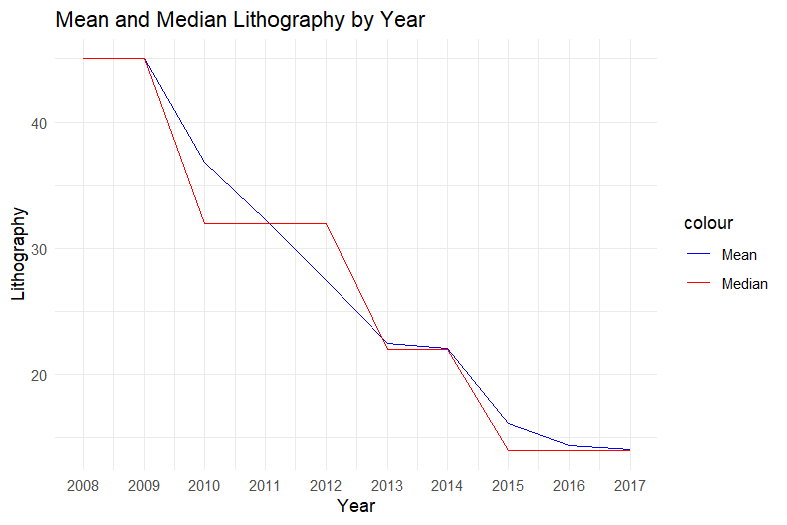
\includegraphics[width=1\linewidth]{img/Litho_Year.png}
  \vspace{1pt}
  \caption{Mean and median of lithography over years}
\end{figure}

\begin{lstlisting}[language=R]
options(repr.plot.width = 15, repr.plot.height =8) 
ggplot(data = CPUs_processed, aes(y = Status, x = Launch_Year, fill = Status)) +
  geom_boxplot() +
  labs(x = "Status", y = "Launch Date",title = "Boxplot of Status over Year") +
  scale_x_continuous(breaks = seq(min(Litho_year$Launch_Year), max(Litho_year$Launch_Year), by = 1))
\end{lstlisting}


\begin{figure}[ht]
  \centering
  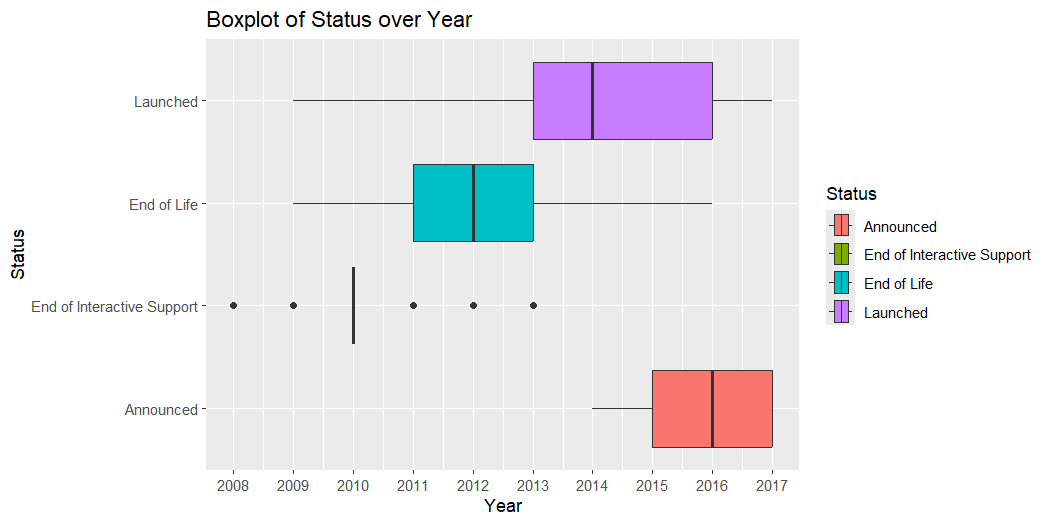
\includegraphics[width=1\linewidth]{img/Status_Year.png}
  \vspace{1pt}
  \caption{Status over years}
\end{figure}

\begin{lstlisting}[language=R]
options(repr.plot.width = 15, repr.plot.height =8) 
ggplot(data = CPUs_processed, aes(y = Vertical_Segment, x = Launch_Year, fill = Vertical_Segment)) +
  geom_boxplot() +
  labs(x = "Year", y = "Vertical Segment",title = "Boxplot of Vertical Segment over Year") +
  scale_x_continuous(breaks = seq(min(Litho_year$Launch_Year), max(Litho_year$Launch_Year), by = 1))
\end{lstlisting}

\begin{figure}[ht]
  \centering
  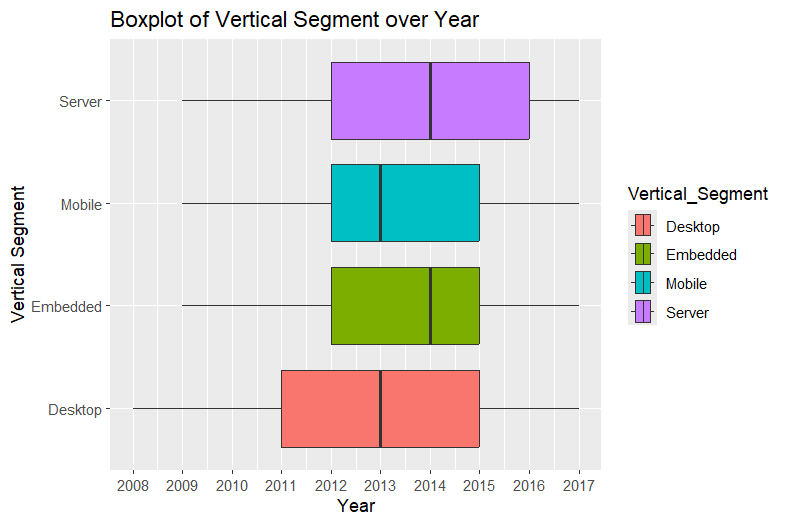
\includegraphics[width=1\linewidth]{img/VSegment_Year.png}
  \vspace{1pt}
  \caption{Segment over years}
\end{figure}

\begin{lstlisting}[language=R]
options(repr.plot.width = 15, repr.plot.height =8) 
ggplot(data = CPUs_processed, aes(y = Instruction_Set, x = Launch_Year, fill = Instruction_Set)) +
  geom_violin() +
  labs(x = "Launch Date", y = "Instruction set",title = "Violinplot of Instruction set over Year") +
  scale_x_continuous(breaks = seq(min(Litho_year$Launch_Year), max(Litho_year$Launch_Year), by = 1))
\end{lstlisting}

\begin{figure}[ht]
  \centering
  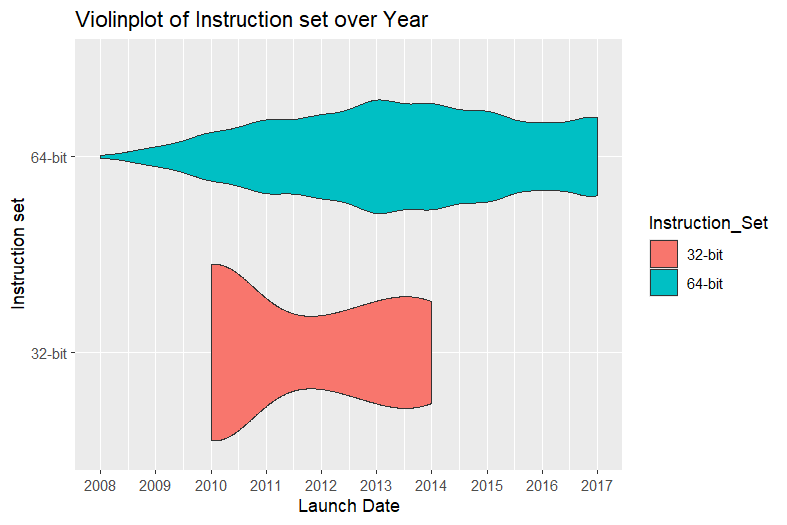
\includegraphics[width=1\linewidth]{img/6432bit_year.png}
  \vspace{1pt}
  \caption{Instruction set over years}
\end{figure}

\begin{figure}[ht]
  \centering
  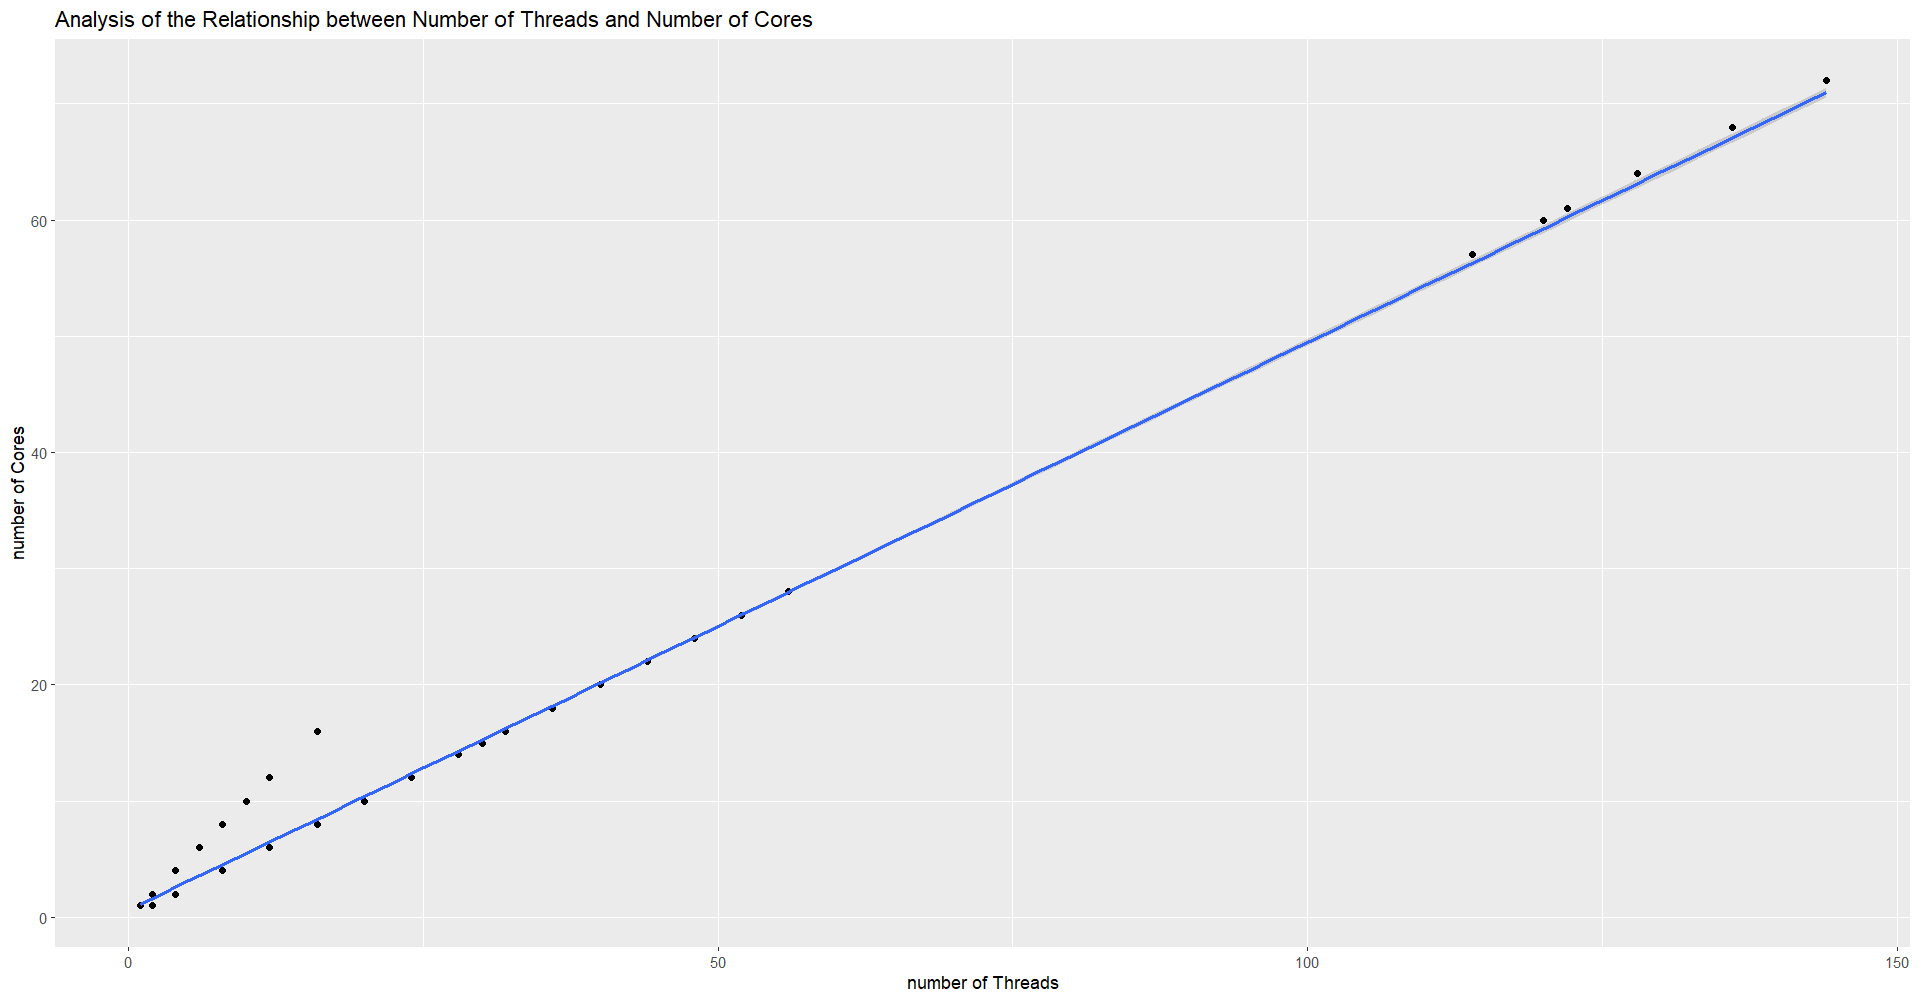
\includegraphics[width=1\linewidth]{img/CPU_ThreadCore.png}
  \vspace{1pt}
  \caption{Relation between Number of Threads and Number of Cores}
\end{figure}

\begin{figure}[ht]
  \centering
  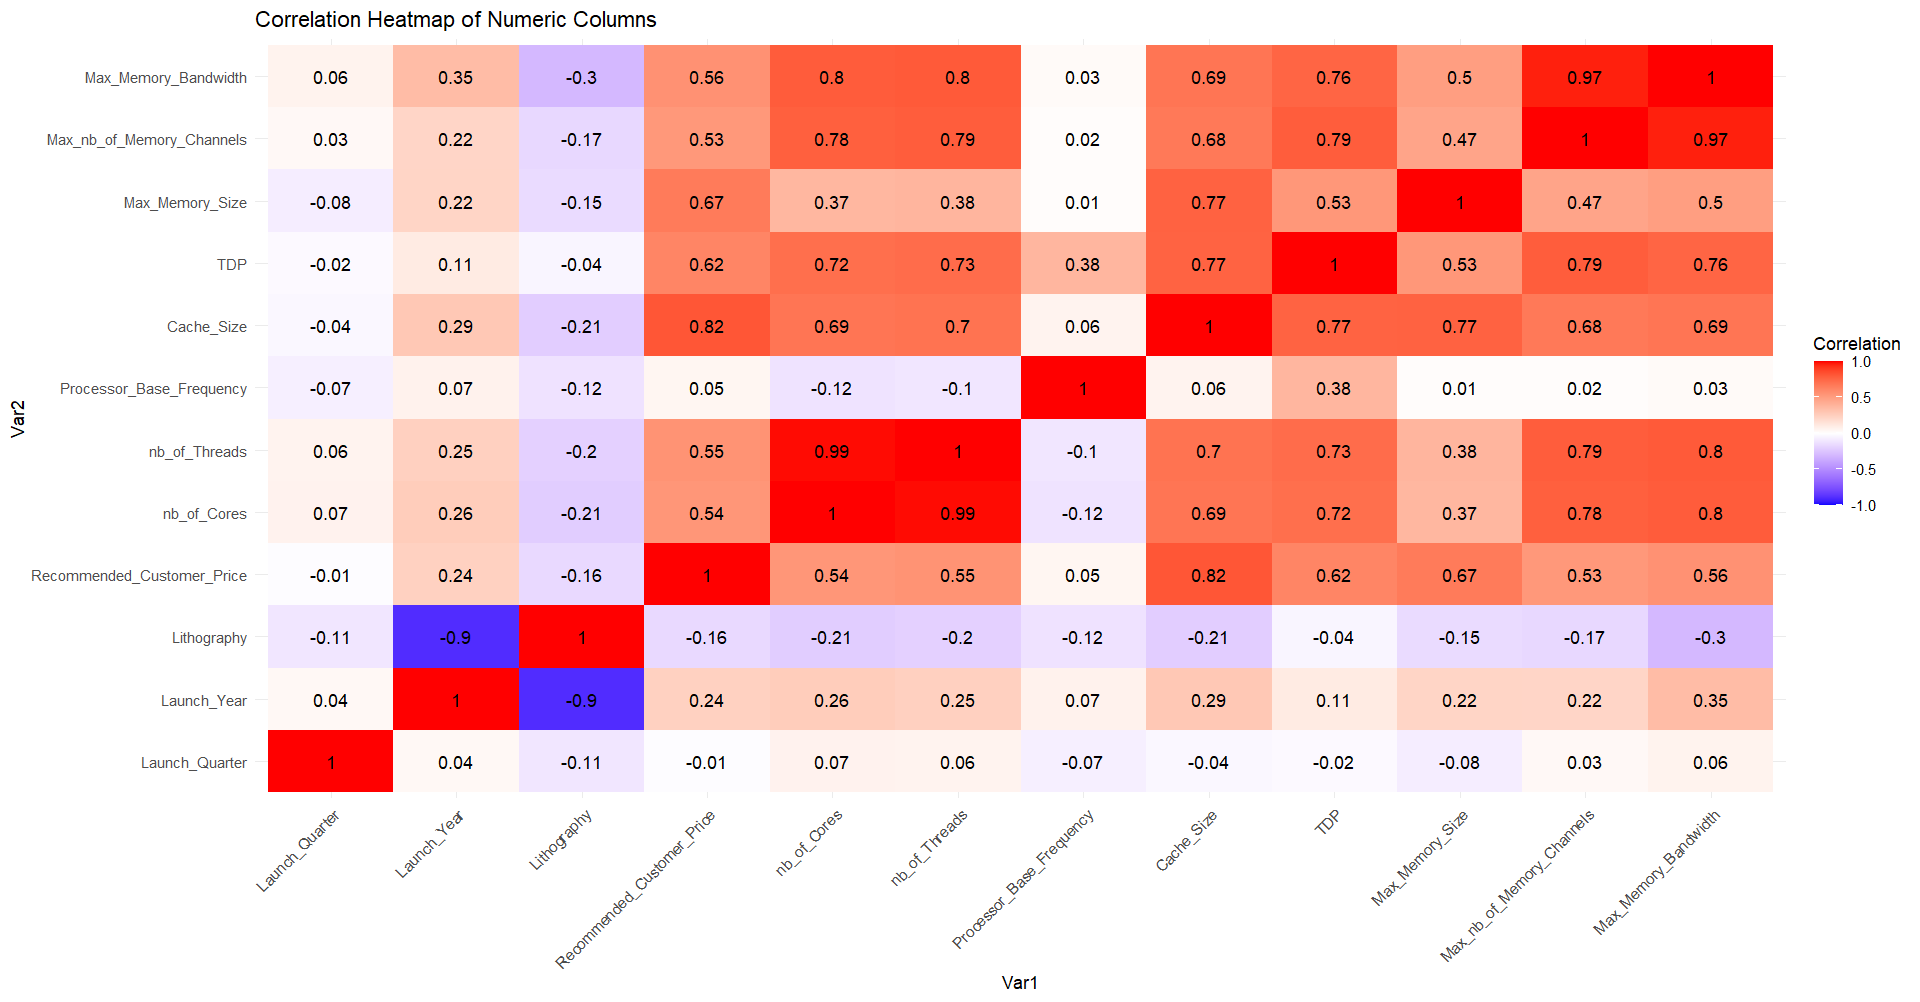
\includegraphics[width=1\linewidth]{img/CPU_cor.png}
  \vspace{1pt}
  \caption{Overall Correlation}
\end{figure}

\section{GPU Data}

\begin{lstlisting}[language=R]
freq <- table(GPUs_processed$Manufacturer, GPUs_processed$Release_Year)
total_count <- colSums(freq)
percentage <- prop.table(freq, margin = 2) * 100

barplot(freq,
        legend.text = TRUE,
        main = "Counts of Each Year",
        xlab = "Year",
        ylab = "Count",
        col = c("skyblue", "salmon", "lightgreen", "yellow"),
        border = "black")
\end{lstlisting}

\begin{figure}[ht]
  \centering
  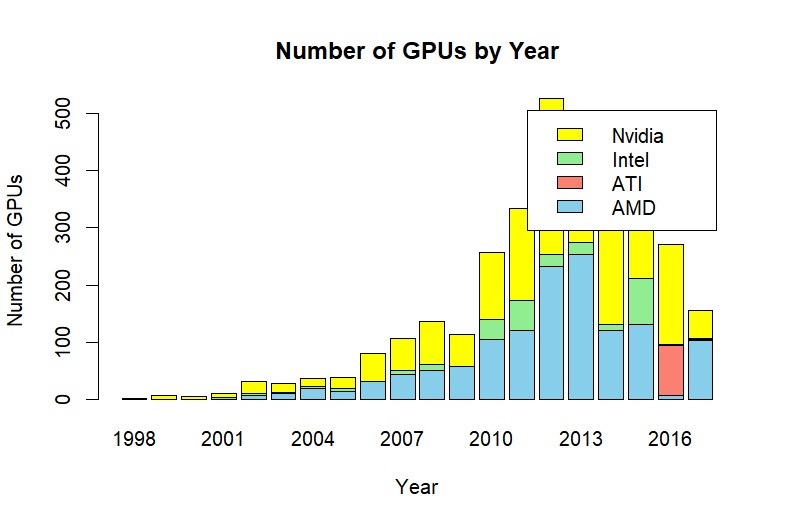
\includegraphics[width=1\linewidth]{img/Market_Year.png}
  \vspace{1pt}
  \caption{Sales of GPU manufacturer over years}
\end{figure}

\begin{lstlisting}[language=R]
barplot(percentage,
        legend.text = TRUE,
        main = "Market Share Percentage by Year",
        xlab = "Year",
        ylab = "Percentage",
        col = c("skyblue", "salmon", "lightgreen", "yellow"),
        border = "black")
\end{lstlisting}

\begin{figure}[ht]
  \centering
  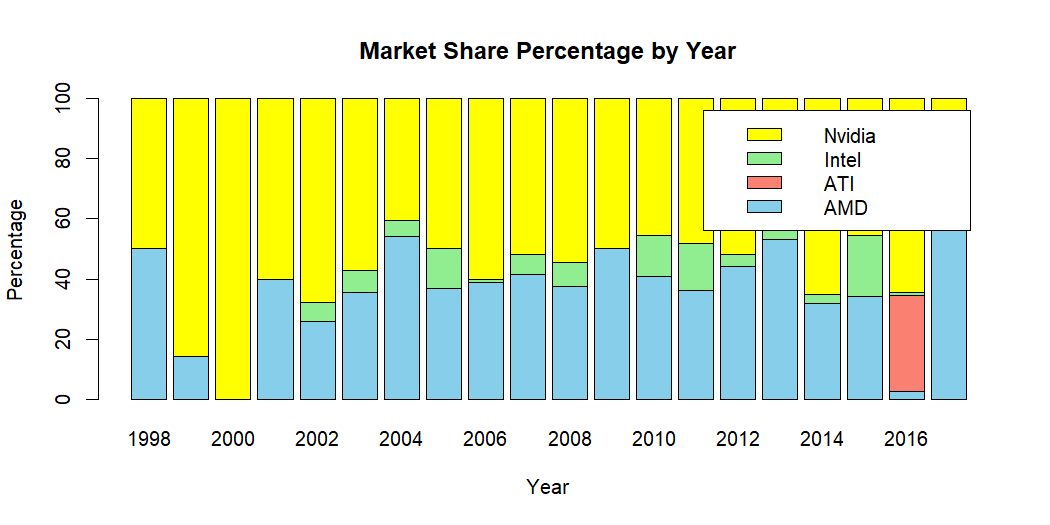
\includegraphics[width=1\linewidth]{img/Market_Percent_Year.png}
  \vspace{1pt}
  \caption{Market Share of GPU manufacturer over years}
\end{figure}

\begin{lstlisting}[language=R]
scatter_plot <- 
  ggplot(GPUs_processed, aes(x = Release_Year + Release_Month/12, y = Memory, color = Manufacturer)) +
  geom_point() +
  scale_color_manual(values = c("skyblue", "salmon", "lightgreen", "yellow")) +
  labs(x = "Year", y = "GPU Memory", title = "Scatter Plot of GPU Memory over Years") +
  theme_minimal()
print(scatter_plot)
\end{lstlisting}

\begin{figure}[ht]
  \centering
  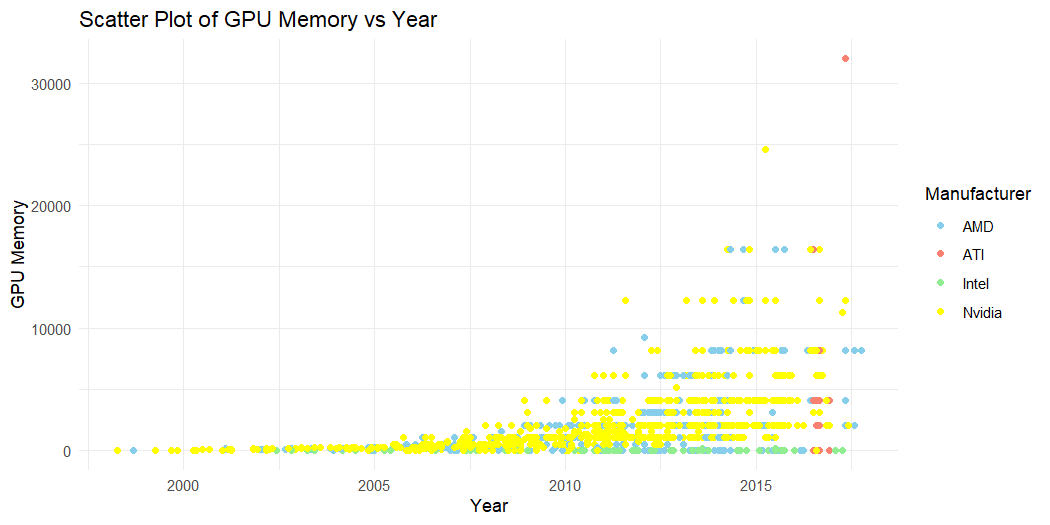
\includegraphics[width=1\linewidth]{img/GPU_Memo_Year.png}
  \vspace{1pt}
  \caption{GPU Memory over Years}
\end{figure}

\begin{lstlisting}[language=R]
memory_summary <- GPUs_processed %>%
  group_by(Release_Year) %>%
  summarise(mean_memory = mean(Memory),
            median_memory = median(Memory))

line_plot <- ggplot(memory_summary, aes(x = Release_Year)) +
  geom_line(aes(y = mean_memory, color = "Mean")) +
  geom_line(aes(y = median_memory, color = "Median")) +
  scale_color_manual(values = c("Mean" = "blue", "Median" = "red")) +
  labs(x = "Year", y = "Memory", title = "Mean and Median Memory by Year") +
  theme_minimal()
print(line_plot)
\end{lstlisting}

\begin{figure}[ht]
  \centering
  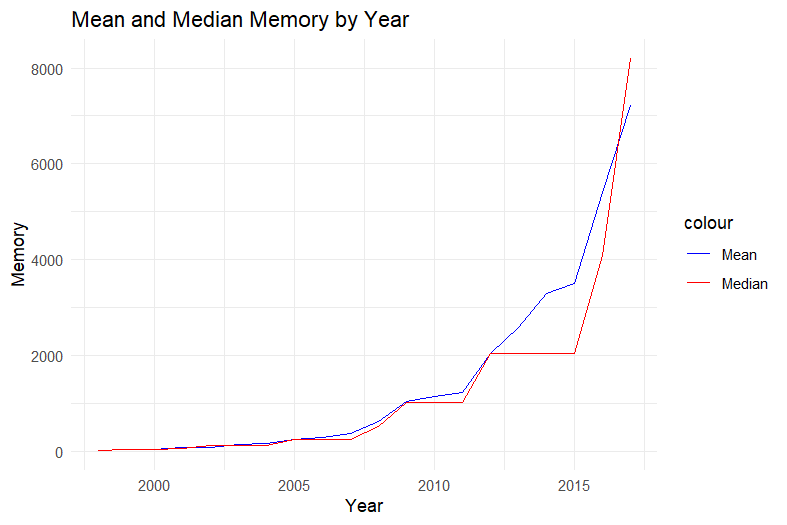
\includegraphics[width=1\linewidth]{img/MeaMedMem_Year.png}
  \vspace{1pt}
  \caption{Mean and median of memory over years}
\end{figure}

\begin{lstlisting}[language=R]
moore_law <- data.frame(
  Release_Year = seq(min(memory_summary$Release_Year), max(memory_summary$Release_Year), 1),
  Memory = 2^(0.5 * (seq(min(memory_summary$Release_Year), max(memory_summary$Release_Year), 1) - min(memory_summary$Release_Year - 8)))
)

memory_summary$log_mean_memory <- log(memory_summary$mean_memory)
memory_summary$log_median_memory <- log(memory_summary$median_memory)

line_plot <- ggplot(memory_summary, aes(x = Release_Year)) +
  geom_line(aes(y = log_mean_memory, color = "Logarithm of Mean"), size = 1) +
  geom_line(aes(y = log_median_memory, color = "Logarithm of Median"), size = 1) +
  geom_line(data = moore_law, aes(y = log(Memory), color = "Moore's Law"), size = 1, linetype = "dashed") +
  scale_color_manual(values = c("Logarithm of Mean" = "blue", "Logarithm of Median" = "red", "Moore's Law" = "green4")) +
  labs(x = "Year", y = "Logarithm of Memory", title = "Logarithm of Mean and Median Memory by Year") +
  theme_minimal()

print(line_plot)
\end{lstlisting}

\begin{figure}[ht]
  \centering
  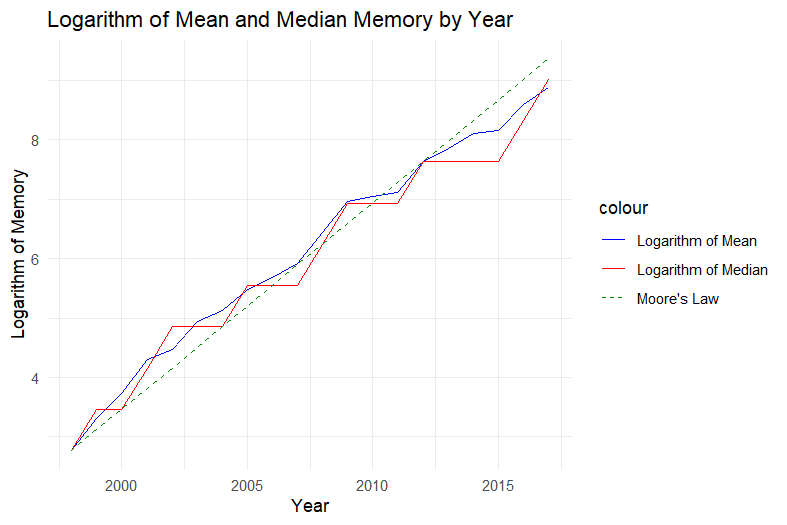
\includegraphics[width=1\linewidth]{img/LogMeaMedMem_Year.png}
  \vspace{1pt}
  \caption{Logarithm of Mean and Median Memory by Year}
\end{figure}


\begin{figure}[ht]
  \centering
  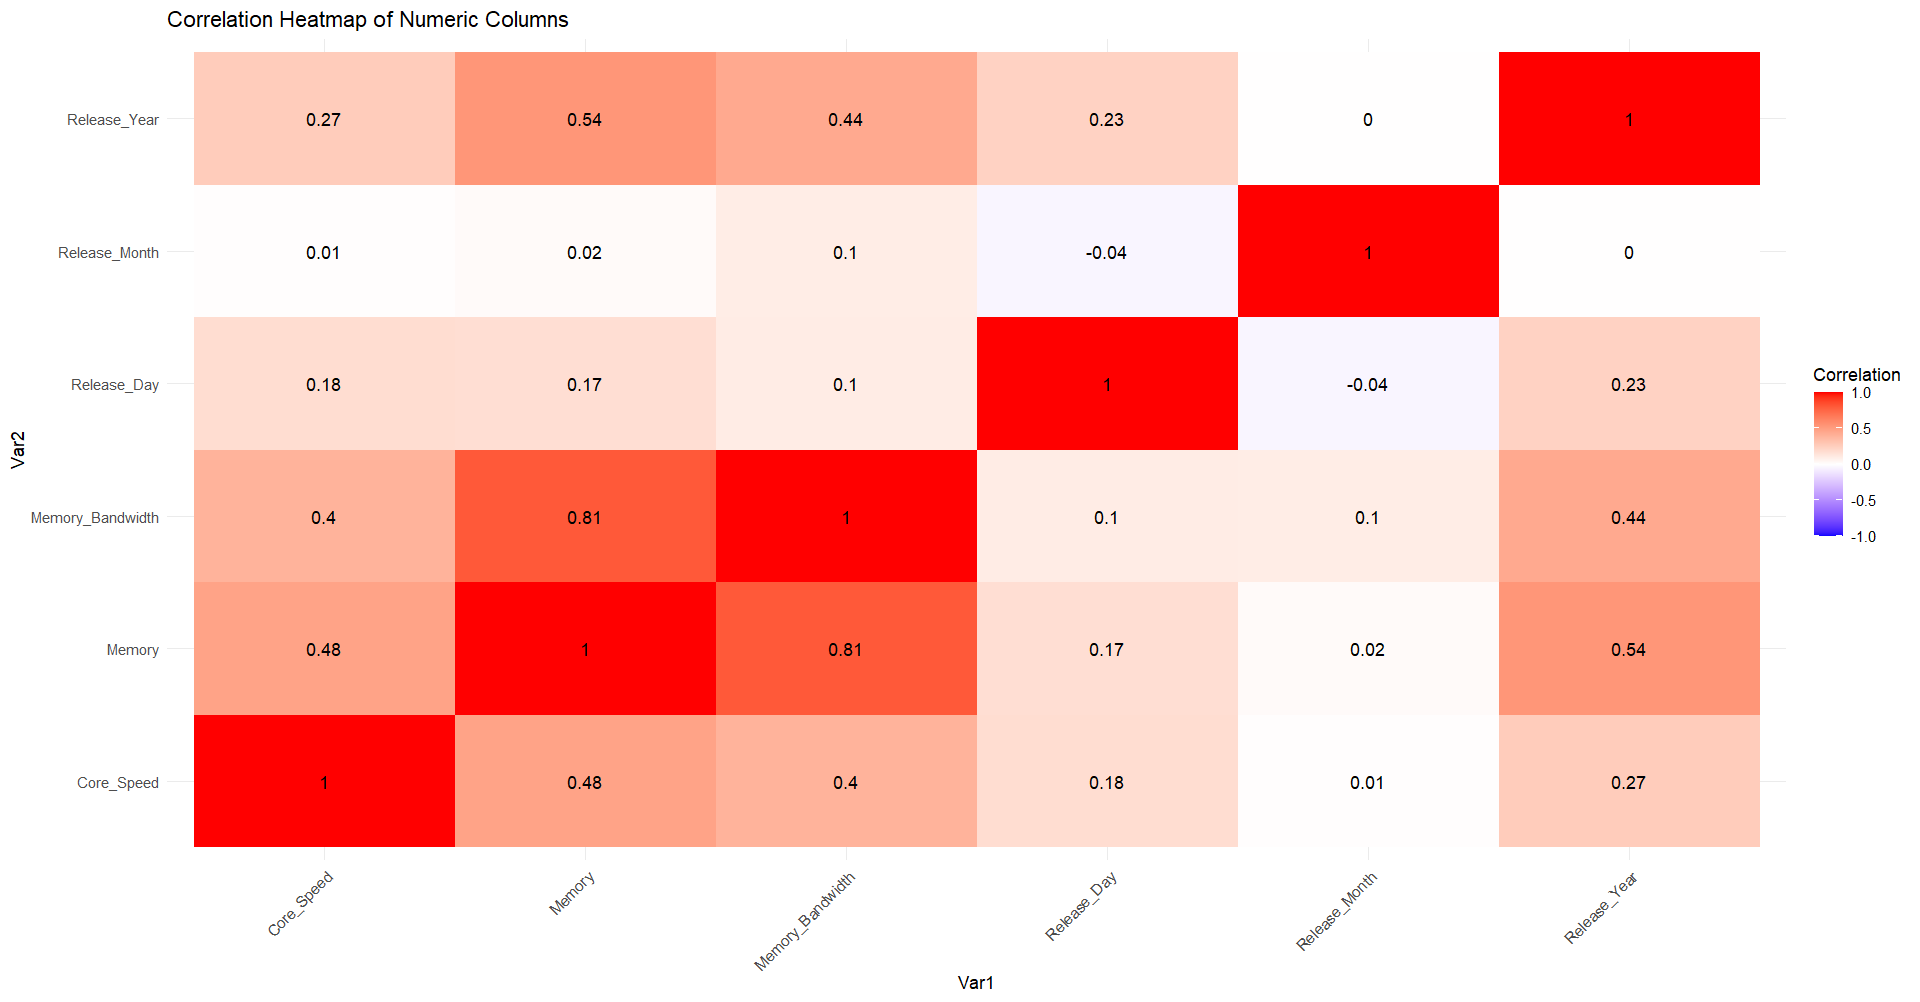
\includegraphics[width=1\linewidth]{img/GPU_cor.png}
  \vspace{1pt}
  \caption{Enter Caption}
\end{figure}